\chapter{Populations and Demography}\label{ch:b1:populations}

A flask of yeast starts with a million \omterm{def:b1:cell-unit-of-life:cell}{cells} and, sixteen hours later,
holds sixty million and has stopped growing; a herd of deer on an
island grows by a tenth each year until the winter its food runs out;
the lynx of the boreal forest rise and crash every ten years, a year
behind the hares they eat. Each is a \emph{\omterm{def:b1:populations:population}{population}} --- the
individuals of one species in one place --- and each obeys arithmetic
that can be written down. This chapter describes how \omterm{def:b1:populations:population}{populations} are
counted, how their births and deaths are tabulated, the two equations
of growth, the forces that hold numbers in check, and what the same
arithmetic says about our own species.

\section{Counting a population}

\begin{definition}[Population, density, dispersion]\label{def:b1:populations:population}
\index{population}\index{population density}
A \emph{population} is the set of individuals of one species living
in a given area at a given time and able to interbreed. Its
\emph{size} $N$ is the number of individuals; its \emph{density} the
number per unit area or volume; its \emph{dispersion} the pattern of
their spacing --- \emph{clumped} where resources or social life gather
them (herds, schools, patches of a plant), \emph{uniform} where they
repel one another (territorial birds, desert shrubs competing for
water), \emph{random} where neither operates. Populations also have an
\emph{age structure}, a \emph{sex ratio}, and rates of birth, death,
immigration and emigration, whose balance is the growth.
\end{definition}

\begin{method}[Estimating a population]\label{met:b1:populations:counting}
\index{mark--recapture}
\begin{enumerate}
  \item Sessile or slow \omterm{def:b1:organism-environment:organism}{organisms}: count in \emph{quadrats} of known
        area placed at random, and multiply the mean density by the
        total area; the scatter among quadrats gives the precision and
        reveals the dispersion.
  \item Mobile animals: \emph{mark--recapture}. Catch $M$
        individuals, mark and release them; later catch $C$, of which
        $R$ are marked. If the marked mix freely and nothing has
        changed, the marked fraction of the second catch equals the
        marked fraction of the \omterm{def:b1:populations:population}{population}, $R/C = M/N$, so
        $N \approx MC/R$ (the Lincoln--Petersen estimate).
  \item Check the assumptions: no births, deaths or migration between
        the catches, marks that neither fall off nor change the
        animal's behaviour, equal catchability. Each failure biases
        $N$ in a predictable direction.
  \item Indirect signs where counting is impossible: droppings,
        tracks, calls, nests, the \omterm{def:b1:nucleic-acids:chain}{DNA} in a litre of pond water.
\end{enumerate}
\end{method}

\begin{example}[Voles in a meadow]\label{ex:b1:populations:voles}
Sixty voles trapped, marked and released in a hectare of meadow;
three nights later eighty are trapped, of which twelve carry marks:
$N \approx 60\times 80/12 = 400$ voles, four per hundred square metres.
If the marked voles, having learned that traps hold food, are caught
more readily, $R$ is inflated and $N$ underestimated; if marking
frightened them away from traps, the reverse.
\end{example}

\section{Demography: births and deaths by age}

\begin{definition}[Life table]\label{def:b1:populations:lifetable}
\index{life table}\index{survivorship}
A \emph{life table} follows a cohort of individuals born together
through their lives. For each age $x$ it records $l_x$, the
\emph{survivorship} --- the fraction of the cohort still alive at age
$x$ --- and $m_x$, the \emph{fecundity} --- the mean number of
daughters born to a female of age $x$. From them: the mortality
between ages, $q_x = 1 - l_{x+1}/l_x$; the \emph{net reproductive
rate} $R_0 = \sum_x l_x m_x$, the number of daughters a newborn female
will have on average in her lifetime; and the \emph{generation time}
$T = \sum_x x\,l_x m_x / R_0$, the mean age of the mothers of those
daughters. A \omterm{def:b1:populations:population}{population} with $R_0 > 1$ grows, with $R_0 < 1$
declines; over one generation it is multiplied by $R_0$.
\end{definition}

\begin{proposition}[Three shapes of survivorship]\label{prop:b1:populations:survivorship}
Plotting $\log l_x$ against age gives three types of curve. \emph{Type
I}: most individuals survive to old age and die within a narrow span
(large mammals, humans in rich countries). \emph{Type II}: a constant
probability of death at every age, a straight line on the log scale
(many birds, lizards, rodents). \emph{Type III}: enormous mortality
among the young and long life for the few survivors (oysters, fish,
most plants and insects). The shape follows from the \omterm{def:b1:organism-environment:organism}{organism}'s way
of life: a species that invests little in each of many offspring has
a type III curve; one that invests much in each of a few, type I.
\end{proposition}

\begin{omfigure}
\begin{tikzpicture}
\begin{semilogyaxis}[
  width=0.86\linewidth, height=6.2cm,
  axis x line=bottom, axis y line=left,
  xmin=0, xmax=100, ymin=1, ymax=1200,
  xlabel={age (\% of maximum lifespan)}, ylabel={survivors per 1000 born},
  xlabel style={font=\small, at={(axis description cs:0.5,-0.12)}, anchor=north},
  ylabel style={font=\small},
  tick label style={font=\small}, xtick={0,25,50,75,100}, ytick={1,10,100,1000}, log ticks with fixed point,
  legend style={font=\small, at={(0.03,0.05)}, anchor=south west, draw=none},
  clip=false,
]
\addplot[very thick, omDef, smooth] coordinates {(0,1000) (20,990) (40,970) (60,900) (75,700) (85,400) (92,150) (97,30) (100,1)};
\addlegendentry{type I: mammals, humans}
\addplot[very thick, omProp, domain=0:100, samples=20] {1000*exp(-0.069*x)};
\addlegendentry{type II: birds, rodents}
\addplot[very thick, omThm, smooth] coordinates {(0,1000) (3,100) (10,15) (25,6) (50,4) (75,2.5) (100,1)};
\addlegendentry{type III: fish, oysters, most plants}
\end{semilogyaxis}
\end{tikzpicture}

{\small Three types of \omterm{def:b1:populations:lifetable}{survivorship} curve, on a logarithmic scale.
Type I dies late, type III dies early, type II dies at a constant
rate; each is a life history written as a line.}
\end{omfigure}

\begin{omfigure}
\begin{tikzpicture}[font=\footnotesize, line cap=round]
  % two age pyramids: growing (left) and stable (right)
  \foreach \i/\m/\f in {0/4.0/3.8, 1/3.4/3.3, 2/2.8/2.7, 3/2.2/2.2, 4/1.6/1.7, 5/1.1/1.2, 6/0.7/0.8, 7/0.35/0.5} {
    \fill[omDef!55] (-\m,0.5*\i) rectangle (0,0.5*\i+0.42);
    \fill[omThm!45] (0,0.5*\i) rectangle (\f,0.5*\i+0.42);
  }
  \node[anchor=north, align=center] at (0,-0.15) {growing population\\ (many young)};
  \foreach \i/\m/\f in {0/1.6/1.5, 1/1.7/1.6, 2/1.8/1.7, 3/1.8/1.8, 4/1.7/1.8, 5/1.5/1.7, 6/1.1/1.4, 7/0.6/0.9} {
    \fill[omDef!55] (8.8-\m,0.5*\i) rectangle (8.8,0.5*\i+0.42);
    \fill[omThm!45] (8.8,0.5*\i) rectangle (8.8+\f,0.5*\i+0.42);
  }
  \node[anchor=north, align=center] at (8.8,-0.15) {stable or ageing population\\ (age classes even)};
  \foreach \i/\l in {0/0--9, 2/20--29, 4/40--49, 6/60--69} { \node[anchor=east, font=\scriptsize] at (-4.3,0.5*\i+0.21) {\l}; }
  \node[anchor=south, omDef!70!black] at (-2.0,4.1) {males}; \node[anchor=south, omThm!80!black] at (2.0,4.1) {females};
\end{tikzpicture}

{\small Age pyramids: the number of individuals in each age class,
males to the left, females to the right. A broad base means many
young and growth to come; even classes mean replacement; a narrow base
means decline.}
\end{omfigure}

\begin{example}[A life table for a deer herd]\label{ex:b1:populations:deer}
Of a thousand fawns, six hundred reach their first birthday, and the
survivors then lose a tenth of their number each year until few pass
nine; does bear from age two, about eight tenths of a daughter a year
in their prime. Summing $l_x m_x$ gives $R_0 \approx 1.5$: each doe
\omterm{def:b1:flowering-plant-organization:organs}{leaves} one and a half daughters, and the herd grows by half each
generation of about four years --- an eleven percent increase per
year until something stops it.
\end{example}

\section{Growth}

\begin{theorem}[Exponential growth]\label{thm:b1:populations:exponential}
\index{exponential growth}\index{intrinsic rate of increase}
A \omterm{def:b1:populations:population}{population} whose per-capita birth and death rates $b$ and $d$ are
constant grows at a rate proportional to its size,
\[
\frac{\dd N}{\dd t} = rN, \qquad r = b - d, \qquad N(t) = N_0\,e^{rt},
\]
where $r$ is the \emph{\omterm{thm:b1:populations:exponential}{intrinsic rate of increase}}. It doubles every
$\ln 2/r$; a \omterm{def:b1:populations:population}{population} with $r = \qty{0.11}{yr^{-1}}$ doubles in
\qty{6.3}{yr}, one with $r = \qty{0.5}{h^{-1}}$ in \qty{83}{min}.
From a \omterm{def:b1:populations:lifetable}{life table}, $r \approx \ln R_0 / T$.
\end{theorem}
\begin{proof}
In a short interval $\dd t$ the births are $bN\,\dd t$ and the deaths
$dN\,\dd t$, so $\dd N = (b - d)N\,\dd t$; the equation
$\dd N/\dd t = rN$ has the solution $N_0 e^{rt}$ (the derivative of
$e^{rt}$ is $re^{rt}$). Doubling: $e^{rt} = 2$ gives $t = \ln 2/r$. Over
one generation $T$ the \omterm{def:b1:populations:population}{population} is multiplied by $R_0 = e^{rT}$,
whence $r = \ln R_0/T$.
\end{proof}

\begin{theorem}[Logistic growth]\label{thm:b1:populations:logistic}
\index{logistic growth}\index{carrying capacity}
If the per-capita growth rate falls linearly as the \omterm{def:b1:populations:population}{population}
approaches a \emph{\omterm{thm:b1:populations:logistic}{carrying capacity}} $K$ --- the size the environment
can sustain ---
\[
\frac{\dd N}{\dd t} = rN\left(1 - \frac{N}{K}\right), \qquad
N(t) = \frac{K}{1 + \dfrac{K - N_0}{N_0}\,e^{-rt}} .
\]
Growth is nearly exponential while $N \ll K$, fastest at $N = K/2$
(where $\dd N/\dd t = rK/4$), and vanishes at $N = K$, which the
\omterm{def:b1:populations:population}{population} approaches as a plateau: an S-shaped curve.
\end{theorem}
\begin{proof}
Write the equation as $\dd N/[N(1 - N/K)] = r\,\dd t$ and split the
left side into $\dd N/N + \dd N/(K - N)$; integrating gives
$\ln[N/(K - N)] = rt + \text{const}$, and solving for $N$ with $N(0) =
N_0$ gives the formula. Differentiating $rN(1 - N/K)$ with respect to
$N$ and setting it to zero gives the maximum at $N = K/2$.
\end{proof}

\begin{omfigure}
\begin{tikzpicture}
\begin{axis}[
  width=0.86\linewidth, height=6.4cm,
  axis x line=bottom, axis y line=left,
  xmin=0, xmax=18, ymin=0, ymax=800,
  xlabel={time (h)}, ylabel={yeast cells per mL ($\times 10^5$)},
  xlabel style={font=\small, at={(axis description cs:0.5,-0.12)}, anchor=north},
  ylabel style={font=\small},
  tick label style={font=\small}, xtick={0,4,8,12,16}, ytick={0,200,400,600,800},
  legend style={font=\small, at={(0.03,0.97)}, anchor=north west, draw=none},
  clip=false,
]
\addplot[very thick, omDef, domain=0:18, samples=100] {660/(1+65*exp(-0.53*x))};
\addlegendentry{logistic, $K = 660$, $r = \qty{0.53}{h^{-1}}$}
\addplot[thick, dashed, omThm, domain=0:9, samples=50, restrict y to domain=0:800] {10*exp(0.53*x)};
\addlegendentry{exponential with the same $r$}
\addplot[only marks, mark=*, mark size=1.8pt, omDef!70!black] coordinates {(0,10) (2,29) (4,71) (6,175) (8,351) (10,513) (12,595) (14,641) (16,656)};
\draw[dashed, gray] (axis cs:0,660) -- (axis cs:18,660); \node[font=\scriptsize, anchor=south east] at (axis cs:18,662) {$K$};
\draw[dashed, gray] (axis cs:0,330) -- (axis cs:7.9,330); \node[font=\scriptsize, anchor=west] at (axis cs:8.2,300) {fastest growth at $K/2$};
\end{axis}
\end{tikzpicture}

{\small A yeast culture counted every two hours (points), the logistic
curve fitted to it, and the exponential it would have followed with no
limit. The two agree for the first six hours and then part.}
\end{omfigure}

\begin{proposition}[Density dependence]\label{prop:b1:populations:densitydependence}
\index{density dependence}
Growth slows as density rises because the per-capita birth rate falls
or the death rate rises with crowding: food per head declines,
territories become unavailable, wastes and disease accumulate,
predators concentrate. These \emph{density-dependent} factors regulate
a \omterm{def:b1:populations:population}{population} toward $K$. \emph{Density-independent} factors --- frost,
flood, fire, drought --- kill a fraction regardless of numbers and
cannot regulate, only disturb; the \omterm{def:b1:populations:population}{populations} of many insects are
governed mostly by the weather and never approach a \omterm{thm:b1:populations:logistic}{carrying capacity}.
\end{proposition}
\begin{proof}[Evidence]
Gause (1934) grew \emph{Paramecium} in tubes of medium renewed daily:
the counts followed a logistic curve to a plateau set by the food,
and doubling the food doubled the plateau. Pearl (1927) found the same
in fruit flies in bottles, and Carlson (1913) in yeast. In the field,
song sparrows on an island lay smaller clutches and lose more young
when the breeding \omterm{def:b1:populations:population}{population} is large, and the number of territories
caps the number of breeders; removing birds is followed by their
replacement from a surplus that had been excluded.
\end{proof}

\begin{definition}[Life-history strategies]\label{def:b1:populations:rK}
\index{r-strategy}\index{K-strategy}
Species differ in where they sit between two extremes. A
\emph{$r$-selected} species --- weeds, aphids, mice, most fish --- is
built for a high $r$: it matures early, produces many small offspring,
invests little in each, lives briefly, and exploits new or disturbed
habitats before the competition arrives, with a type III \omterm{def:b1:populations:lifetable}{survivorship}.
A \emph{$K$-selected} species --- oaks, elephants, albatrosses ---
is built to persist near $K$: it matures late, produces few large
offspring, cares for them, lives long, competes well in crowded
stable habitats, with a type I curve. Most species mix the two; the
labels name the ends of the scale.
\end{definition}

\section{Fluctuation and regulation}

\begin{proposition}[Cycles of predator and prey]\label{prop:b1:populations:cycles}
\index{population cycle}
Some \omterm{def:b1:populations:population}{populations} do not settle but oscillate. The snowshoe hare of
the northern forest and the lynx that eats it rise and fall together
with a period of about ten years, the lynx a year or two behind the
hare: many hares feed many lynx, many lynx eat the hares down, few
hares starve the lynx, few lynx let the hares recover. The cycle is
driven partly by the predator and partly by the hares' own food, whose
recovery after overbrowsing takes years; models of coupled predator
and prey (\cref{ch:b1:species-interactions}) reproduce such
oscillations from two equations.
\end{proposition}
\begin{proof}[Evidence]
The fur returns of a trading company, kept for ninety years from the
1840s, record the number of lynx and hare pelts brought in each year
across a subcontinent: both series show peaks every nine to ten years,
the lynx peak lagging the hare's, over nine full cycles. Field studies
since, with hares fenced from predators or given extra food, show
that removing either factor damps the cycle and removing both
abolishes it.
\end{proof}

\begin{omfigure}
\begin{tikzpicture}
\begin{axis}[
  width=0.9\linewidth, height=6.0cm,
  axis x line=bottom, axis y line=left,
  xmin=1845, xmax=1935, ymin=0, ymax=160,
  xlabel={year}, ylabel={pelts traded (thousands)},
  xlabel style={font=\small, at={(axis description cs:0.5,-0.12)}, anchor=north},
  ylabel style={font=\small},
  tick label style={font=\small, /pgf/number format/1000 sep=}, xtick={1850,1870,1890,1910,1930}, ytick={0,50,100,150},
  legend style={font=\small, at={(0.97,0.97)}, anchor=north east, draw=none},
  clip=false,
]
\addplot[very thick, omProp, smooth] coordinates {(1845,20) (1848,50) (1851,120) (1853,40) (1856,15) (1859,60) (1862,140) (1864,60) (1867,20) (1870,50) (1873,100) (1876,30) (1879,12) (1882,70) (1885,150) (1888,40) (1891,20) (1894,50) (1897,100) (1900,30) (1903,15) (1906,60) (1909,120) (1912,30) (1915,15) (1918,50) (1921,110) (1924,40) (1927,15) (1930,60) (1933,100)};
\addlegendentry{snowshoe hare}
\addplot[very thick, omDef, smooth] coordinates {(1845,10) (1849,20) (1852,45) (1855,20) (1858,8) (1861,25) (1864,60) (1866,25) (1869,10) (1872,30) (1875,40) (1878,15) (1881,10) (1884,40) (1887,70) (1890,20) (1893,10) (1896,30) (1899,45) (1902,15) (1905,8) (1908,35) (1911,55) (1914,15) (1917,8) (1920,30) (1923,50) (1926,15) (1929,10) (1932,30) (1935,45)};
\addlegendentry{lynx}
\end{axis}
\end{tikzpicture}

{\small Hare and lynx pelts brought to the trading posts of the
northern forest, year by year (smoothed). Both cycle with a period of
about ten years, the lynx a year or two behind the hare.}
\end{omfigure}

\begin{omfigure}
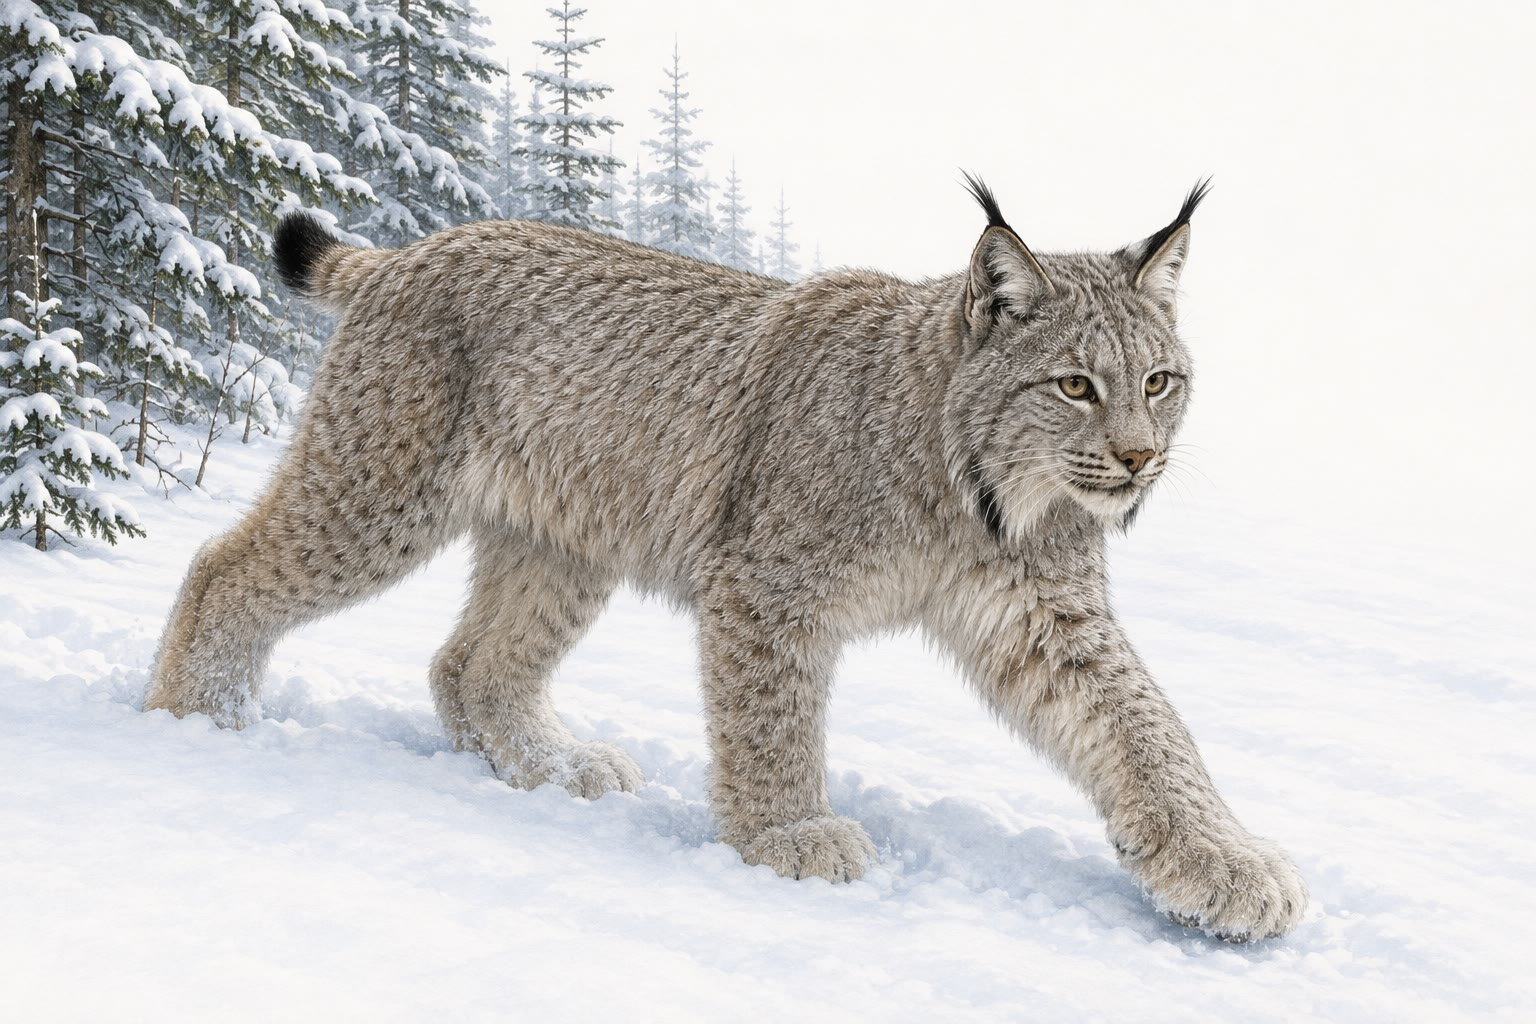
\includegraphics[width=0.52\linewidth]{images/book3/ai/b3-25-lynx-snow.jpg}

{\small A lynx in the boreal forest. Its numbers follow the hare's
with a lag: the predator's cycle is the prey's, delayed.}
\end{omfigure}

\begin{example}[Our own species]\label{ex:b1:populations:humans}
The human \omterm{def:b1:populations:population}{population} took all of history to reach one billion, in
about 1800, and two centuries to reach eight. Its growth rate peaked
near \qty{2}{\%} a year in the 1960s (doubling in 35 years) and has
since fallen below \qty{1}{\%}, not through deaths but through births:
where child mortality falls and women are educated, families shrink
within a generation, and the age pyramid turns from a triangle to a
column. The arithmetic of $R_0$ applies to us; what changed is $m_x$.
\end{example}

\section{Exercises}

\begin{exercise}[$\star$]\label{exo:b1:populations:1}
Define \omterm{def:b1:populations:population}{population}, density and dispersion, and give an example of
each pattern of dispersion.
\end{exercise}

\begin{exercise}[$\star$]\label{exo:b1:populations:2}
Define $l_x$, $m_x$, $R_0$ and $T$, and say what $R_0 = 1$ means.
\end{exercise}

\begin{exercise}[$\star$]\label{exo:b1:populations:3}
From the \omterm{def:b1:populations:lifetable}{survivorship} figure, what fraction of a type III cohort
survives the first tenth of its lifespan? Of a type I cohort, what
fraction reaches three quarters of it?
\end{exercise}

\begin{exercise}[$\star$]\label{exo:b1:populations:4}
State the exponential and logistic equations and say what $r$ and $K$
mean.
\end{exercise}

\begin{exercise}[$\star\star$]\label{exo:b1:populations:5}
A bacterial culture grows from $10^4$ to $10^7$ \omterm{def:b1:cell-unit-of-life:cell}{cells} per millilitre
in \qty{5}{h}. Compute $r$ and the doubling time.
\end{exercise}

\begin{exercise}[$\star\star$]\label{exo:b1:populations:6}
A \omterm{def:b1:populations:lifetable}{life table}: $l_x = 1, 0.5, 0.3, 0.1, 0$ at ages 0 to 4; $m_x = 0,
1, 2, 2, 0$. Compute $R_0$, $T$ and $r$, and say whether the
\omterm{def:b1:populations:population}{population} grows.
\end{exercise}

\begin{exercise}[$\star\star$]\label{exo:b1:populations:7}
Fifty fish are marked and released in a pond; a week later 70 are
caught, 7 marked. Estimate $N$. If ten of the marked fish died of the
handling, is the estimate too high or too low, and by how much?
\end{exercise}

\begin{exercise}[$\star\star$]\label{exo:b1:populations:8}
A logistic \omterm{def:b1:populations:population}{population} has $K = 1000$ and $r = \qty{0.2}{yr^{-1}}$.
Compute $\dd N/\dd t$ at $N = 100$, $500$ and $900$, and the maximum
number that can be harvested each year without decline.
\end{exercise}

\begin{exercise}[$\star\star$]\label{exo:b1:populations:9}
Classify as $r$- or $K$-selected, with two traits each: a dandelion,
an elephant, a cod, a gorilla, a housefly.
\end{exercise}

\begin{exercise}[$\star\star\star$]\label{exo:b1:populations:10}
From the yeast figure, estimate $r$ from the first two points and $K$
from the last, then predict $N$ at \qty{8}{h} from the logistic
formula and compare with the count. At what time is the growth rate
highest, and what is it?
\end{exercise}

\begin{exercise}[$\star\star\star$]\label{exo:b1:populations:11}
Explain why a density-independent factor cannot regulate a \omterm{def:b1:populations:population}{population}
although it can reduce it, using the equations, and why insect
\omterm{def:b1:populations:population}{populations} governed by weather nonetheless do not grow without
limit.
\end{exercise}

\begin{exercise}[$\star\star\star$]\label{exo:b1:populations:12}
``A \omterm{def:b1:populations:population}{population} is not a number but a distribution.'' Discuss in a
paragraph: age structure, the lag between a fall of $m_x$ and a fall
of $N$, and what a pyramid predicts that $N$ alone does not.
\end{exercise}

\section{Problem: Yeast in a Flask and Deer on an Island}

\begin{problem}[{Weekend problem --- a culture counted, a herd
tabulated, a lake sampled and a harvest set, ending on the carrying
capacity and intrinsic growth rate of the yeast}]
\label{pb:b1:populations:1}
A yeast culture is counted every two hours (\omterm{def:b1:cell-unit-of-life:cell}{cells} per millilitre,
$\times 10^5$): $10, 29, 71, 175, 351, 513, 595, 641, 656$ at $t = 0,
2, \ldots, 16$ h. A deer \omterm{def:b1:populations:population}{population} on an island has the \omterm{def:b1:populations:lifetable}{life table}:
$l_x = 1.00, 0.60, 0.52, 0.46, 0.40, 0.34, 0.26, 0.16, 0.06, 0$ and
$m_x = 0, 0, 0.6, 0.8, 0.8, 0.8, 0.7, 0.5, 0.3, 0$ for $x = 0$ to $9$
years. In a lake, 120 perch are marked and released; a week later 150
are caught, 18 marked.

\medskip
\noindent\textbf{Part I --- The yeast.}
\begin{enumerate}
  \item Estimate $r$ from the first two counts, assuming \omterm{thm:b1:populations:exponential}{exponential
        growth} over the first two hours.
  \item Compute the doubling time.
  \item Estimate $K$ from the last counts.
  \item Compute the logistic prediction at $t = 4$, $8$ and \qty{12}{h}
        and compare with the counts.
  \item At what \omterm{def:b1:populations:population}{population} is growth fastest, and when is it reached?
        Compute the maximum growth rate in \omterm{def:b1:cell-unit-of-life:cell}{cells} per millilitre per
        hour.
  \item What would the exponential model predict at \qty{12}{h}? By
        what factor is it wrong?
  \item Name two things that could set $K$ in a sealed flask of
        yeast.
\end{enumerate}

\medskip
\noindent\textbf{Part II --- The deer.}
\begin{enumerate}[resume]
  \item Compute the mortality $q_x$ in the first year and in the fifth.
        Which \omterm{def:b1:populations:lifetable}{survivorship} type is this?
  \item Compute $l_x m_x$ for each age and sum them: $R_0$.
  \item Compute $T$.
  \item Compute $r$ and the doubling time of the herd.
  \item The island holds 200 deer today. Predict the number in 10
        years by \omterm{thm:b1:populations:exponential}{exponential growth}.
  \item The island can feed 600 deer. Predict the number in 10 years by
        \omterm{thm:b1:populations:logistic}{logistic growth}, and the year in which the herd passes 500.
\end{enumerate}

\medskip
\noindent\textbf{Part III --- The perch and the harvest.}
\begin{enumerate}[resume]
  \item Estimate the perch \omterm{def:b1:populations:population}{population} of the lake.
  \item If 20 of the marked perch lost their marks before the second
        catch, recompute with the true number of marked fish, and
        state the direction of the error in the first estimate.
  \item The perch \omterm{def:b1:populations:population}{population} has $K = 1000$ and $r = \qty{0.4}{yr^{-1}}$.
        Compute the maximum sustainable yield and the \omterm{def:b1:populations:population}{population} at
        which it is obtained.
  \item Compute the doubling time of the perch \omterm{def:b1:populations:population}{population} when it is
        far below $K$.
  \item The club decides instead to take a fixed \qty{20}{\%} of the
        stock each year. Compute the equilibrium \omterm{def:b1:populations:population}{population} and the
        yearly catch at that equilibrium.
  \item An angler's club takes 120 perch a year. Show whether the
        \omterm{def:b1:populations:population}{population} can sustain it, by computing $\dd N/\dd t$ at $N =
        500$ and at $N = 300$.
  \item Why is harvesting at $K/2$ risky in practice, with the
        weather and the counting error of question 14 in mind?
\end{enumerate}

\medskip
\noindent\textbf{Part IV --- Regulation.}
\begin{enumerate}[resume]
  \item The deer's $m_x$ falls to half when the herd exceeds 400. Show
        that $R_0$ then drops below 1 --- what does this do to the
        herd, and what kind of factor is at work?
  \item A hard winter kills \qty{40}{\%} of the deer regardless of
        their number. Is this factor regulating? What happens to the
        herd in the years after?
  \item Wolves arrive and take a fixed 30 deer a year. Compute the
        equilibrium herd sizes for the logistic model with $K = 600$
        and the $r$ of question 11 (solve $rN(1 - N/K) = 30$), and
        say which equilibrium is stable.
  \item Explain in two sentences why the lynx cycle lags the hare's.
  \item State the result: the \omterm{thm:b1:populations:logistic}{carrying capacity} and intrinsic growth
        rate of the yeast, and $R_0$, $T$ and $r$ of the deer.
\end{enumerate}
\end{problem}
